




\section{Additional Experimental Details and Results}
\label{sec:experimental-setup}

\subsection{Hyperparameter Tuning}
\label{sec:hyperp-tuning}

DP-SGD and DP-CD both depend on three hyperparameters: step size,
clipping threshold and number of passes on data. For DP-CD, step sizes
are adapted from a parameter as described in
\Cref{sec:numerical-experiments}, and clipping thresholds as well (see \Cref
{sub:clipping}). For DP-SGD, the step size is given by $\gamma/\beta$,
where $\gamma$ is the hyperparameter and $\beta$ is the problem's global
smoothness constant  (which we consider given), and the clipping threshold is
used directly to clip gradients along their $\ell_2$-norm.

We simultaneously tune these three hyperparameters for each algorithm across
the following grid:
\begin{itemize}
\item step size: 10 logarithmically-spaced values between $10^{-6}$
  and $1$ for DP-SGD, and between $10^{-2}$ and $10$ for DP-CD.\footnote{Recall that step sizes for CD algorithms are coordinate-wise, and
  thus larger than in SGD algorithms. We empirically verify that
  the best
  step size always lies strictly inside the considered interval for both
  DP-CD and DP-SGD.}
\item clipping threshold: 100 logarithmically-spaced values, between
  $10^{-3}$ and $10^{6}$.
\item number of passes: 5 values (2, 5, 10, 20 and 50).
\end{itemize}
We run each algorithm on each dataset 5~times on each combination of
hyperparameter values.  We then keep the set of hyperparameters that
yield the lowest value of the objective at the last iterate, averaged
across the $5$~runs.

In \Cref{tab:full-tuning-max-iter}, we report the best relative error
(in comparison to optimal objective value) at the last iterate,
averaged over five runs, for each dataset, algorithm, and total number
of passes on the data. As such, each cell of this table corresponds to
the best value obtained after tuning the step size and clipping
hyperparameters for a given number of passes.

\begin{table}[t]
  \centering
  \scriptsize

  \caption{
    Relative error to non-private optimal value of the
    objective function for different number of passes on the
    data. Results are reported for each dataset and for DP-CD and
    DP-SGD, after tuning step size and clipping
    hyperparameters. A star indicates the lowest error in each row.
  }

  \label{tab:full-tuning-max-iter}
  \begin{tabular}{ccccccc}
    \toprule
    & Passes on data &2  	 &5  	 &10  	 &20  	 &50  	 \\
    \midrule
    Electricity (imbalanced) & DP-CD  & $ 0.1458 \pm 6\text{e-}04 $ 	 & $ 0.0842 \pm 1\text{e-}03 $ 	 & $ 0.0436 \pm 2\text{e-}03 $ 	 & $ 0.0147 \pm 2\text{e-}03 $ 	 & $ 0.0020 \pm 1\text{e-}03 $* 	 \\
    $\epsilon=1, \delta=1/n^2$ & DP-SGD  & $ 0.2047 \pm 2\text{e-}02 $ 	 & $ 0.1804 \pm 2\text{e-}02 $ 	 & $ 0.1766 \pm 2\text{e-}02 $ 	 & $ 0.1644 \pm 2\text{e-}02 $ 	 & $ 0.1484 \pm 1\text{e-}02 $* 	 \\
    \midrule
    Electricity (balanced) & DP-CD  & $ 0.0186 \pm 4\text{e-}04 $ 	 & $ 0.0023 \pm 4\text{e-}04 $ 	 & $ 0.0013 \pm 6\text{e-}04 $* 	 & $ 0.0013 \pm 4\text{e-}04 $ 	 & $ 0.0019 \pm 8\text{e-}04 $ 	 \\
    $\epsilon=1, \delta=1/n^2$ & DP-SGD  & $ 0.0391 \pm 1\text{e-}02 $ 	 & $ 0.0189 \pm 5\text{e-}03 $ 	 & $ 0.0123 \pm 4\text{e-}03 $ 	 & $ 0.0106 \pm 3\text{e-}03 $ 	 & $ 0.0040 \pm 2\text{e-}03 $* 	 \\
    \midrule
    California (imbalanced) & DP-CD  & $ 0.1708 \pm 7\text{e-}03 $ 	 & $ 0.1232 \pm 1\text{e-}02 $ 	 & $ 0.0598 \pm 1\text{e-}02 $ 	 & $ 0.0287 \pm 5\text{e-}03 $ 	 & $ 0.0124 \pm 7\text{e-}03 $* 	 \\
    $\epsilon=1, \delta=1/n^2$ & DP-SGD  & $ 0.2799 \pm 9\text{e-}02 $ 	 & $ 0.1863 \pm 2\text{e-}02 $ 	 & $ 0.1476 \pm 2\text{e-}02 $ 	 & $ 0.1094 \pm 2\text{e-}02 $ 	 & $ 0.1068 \pm 2\text{e-}02 $* 	 \\
    \midrule
    California (balanced) & DP-CD  & $ 0.0007 \pm 3\text{e-}04 $* 	 & $ 0.0011 \pm 6\text{e-}04 $ 	 & $ 0.0012 \pm 5\text{e-}04 $ 	 & $ 0.0010 \pm 1\text{e-}04 $ 	 & $ 0.0017 \pm 1\text{e-}03 $ 	 \\
    $\epsilon=1, \delta=1/n^2$ & DP-SGD  & $ 0.0351 \pm 2\text{e-}02 $ 	 & $ 0.0226 \pm 8\text{e-}03 $ 	 & $ 0.0125 \pm 3\text{e-}03 $ 	 & $ 0.0087 \pm 2\text{e-}03 $ 	 & $ 0.0042 \pm 1\text{e-}03 $* 	 \\
    \midrule
    Sparse LASSO & DP-CD  & $ 0.2498 \pm 4\text{e-}02 $* 	 & $ 0.4702 \pm 9\text{e-}02 $ 	 & $ 0.5982 \pm 4\text{e-}02 $ 	 & $ 0.7160 \pm 2\text{e-}02 $ 	 & $ 0.7551 \pm 0\text{e+}00 $ 	 \\
    $\epsilon=10, \delta=1/n^2$ & DP-SGD  & $ 0.7551 \pm 0\text{e+}00 $ 	 & $ 0.7551 \pm 3\text{e-}09 $* 	 & $ 0.7551 \pm 0\text{e+}00 $ 	 & $ 0.7551 \pm 0\text{e+}00 $ 	 & $ 0.7551 \pm 0\text{e+}00 $ 	 \\
    \bottomrule



  \end{tabular}
\end{table}

\subsection{Running Time}
\label{sec:running-time-in}

\begin{figure}[t]
  \captionsetup[subfigure]{justification=centering}
  \centering
  \begin{subfigure}{0.045\linewidth}
    \centering
    \includegraphics[width=\linewidth]{plots/xlegend.pdf}
    \begin{minipage}{.1cm}
      \vfill
    \end{minipage}
  \end{subfigure}%
  \begin{subfigure}{0.3\linewidth}
    \centering
    \includegraphics[width=\linewidth]{plots/time_optimization_electricity_raw.pdf}
    \caption{Electricity (logistic).\\ Imbalanced.}
    \label{fig:expe-time-electricity-raw}
  \end{subfigure}%
  \begin{subfigure}{0.3\linewidth}
    \centering
    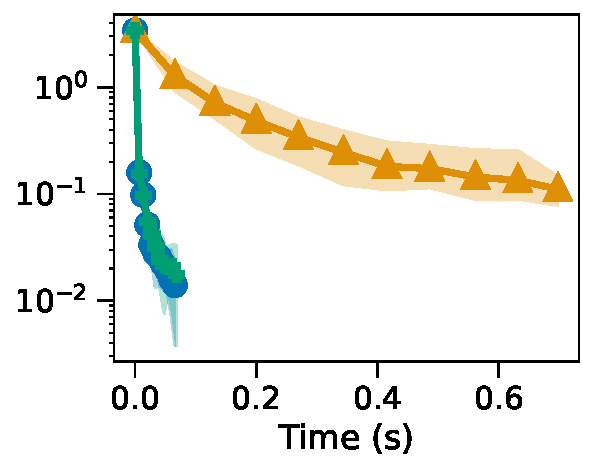
\includegraphics[width=\linewidth]{plots/time_optimization_california_raw.pdf}
    \caption{California (LASSO).\\ Imbalanced.}
    \label{fig:expe-time-california-raw}
  \end{subfigure}
  \begin{subfigure}{0.045\linewidth}
    \centering
    \includegraphics[width=\linewidth]{plots/xlegend.pdf}
    \begin{minipage}{.1cm}
      \vfill
    \end{minipage}
  \end{subfigure}%
  \begin{subfigure}{0.3\linewidth}
    \centering
    \includegraphics[width=\linewidth]{plots/time_optimization_electricity_norm.pdf}
    \caption{Electricity (logistic).\\ Balanced.}
    \label{fig:expe-time-electricity-norm}
  \end{subfigure}%
  \begin{subfigure}{0.3\linewidth}
    \centering
    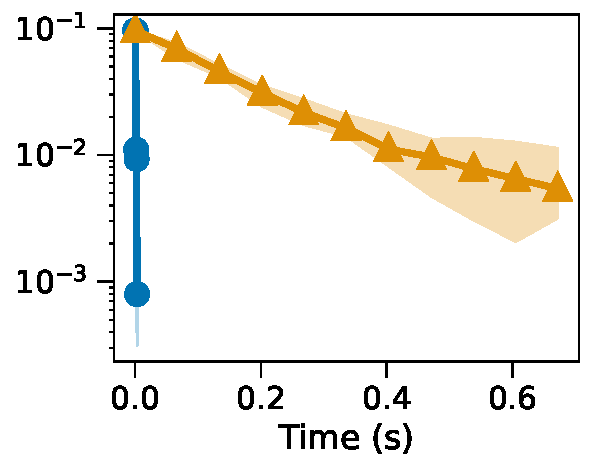
\includegraphics[width=\linewidth]{plots/time_optimization_california_norm.pdf}
    \caption{California (LASSO).\\ Balanced.}
    \label{fig:expe-time-california-norm}
  \end{subfigure}
  \begin{subfigure}{0.3\linewidth}
    \centering
    \includegraphics[width=\linewidth]{plots/time_optimization_lasso.pdf}
    \caption{Sparse LASSO.\\ Balanced.}
    \label{fig:expe-time-lasso}
  \end{subfigure}


  \caption{Relative error to non-private optimal for DP-CD (blue,
    round marks), DP-CD with privately estimated coordinate-wise smoothness
    constants (green, + marks) and DP-SGD (orange, triangle marks) on
    five problems. We report average, minimum and maximum values over
    10~runs for each algorithm, as a function of the algorithm running
    time (in seconds).  }
  \label{fig:expe-time}
\end{figure}

\aurelien{say something about the implementation (and recall it is included
as supplementary material), and the machine on which the experiments are run.}

In this section, we report the running times of DP-CD and DP-SGD.  We
implemented DP-CD and DP-SGD in C++, with Python bindings\footnote{The
  code is available at
  \url{https://gitlab.inria.fr/pmangold1/private-coordinate-descent/}.}. The
design matrix and the labels are kept in memory as dense matrices of
the Eigen library. No special code optimization nor tricks is applied
to the algorithms, except for the update of residuals at each
iteration of DP-CD, which prevents from accessing the complete dataset
at each step. All experiments were run on a laptop with 16GB of RAM
and an Intel(R) Core(TM) i7-10610U CPU @ 1.80GHz.

\Cref{fig:expe-time} shows the same experiments as in
\Cref{fig:expe-raw} and \Cref{fig:expe-standardized}, but as a
function of the running time. In our implementation, DP-CD runs about
$4$ times as fast as DP-SGD for a given number of iterations (see
\Cref{fig:expe-time-electricity-raw} and
\Cref{fig:expe-time-california-raw} for $50$ iterations). On the three
other plots, \Cref{fig:expe-time-electricity-norm},
\Cref{fig:expe-time-california-norm} and \Cref{fig:expe-time-lasso},
DP-CD yields better results in less iterations. DP-CD is thus
particularly valuable in these scenarios: combined with its faster
running time, it provides accurate results extremely fast.  For
completeness, we provide in \Cref{tab:full-tuning-runtime} the full
table of running time, corresponding to
\Cref{tab:full-tuning-max-iter} and \Cref{fig:expe-time}. These
results show that, for a given number of passes on the data, DP-CD
consistently runs about $5$ times faster than DP-SGD.


\begin{table}[H]
  \centering
  \scriptsize

  \caption{ Time of execution (in seconds) for different number of
    passes on the data (averaged over 10~runs). Results are reported
    for each dataset and for DP-CD and DP-SGD, after tuning step size
    and clipping hyperparameters.
  }

  \label{tab:full-tuning-runtime}
  \begin{tabular}{ccccccc}
    \toprule
    & Passes on data &2  	 &5  	 &10  	 &20  	 &50  	 \\
    \midrule
    Electricity (imbalanced) & DP-CD & $ 0.0128 \pm 1\text{e-}03 $ 	 & $ 0.0274 \pm 1\text{e-}03 $ 	 & $ 0.0500 \pm 1\text{e-}03 $ 	 & $ 0.0980 \pm 7\text{e-}04 $ 	 & $ 0.2457 \pm 2\text{e-}03 $ 	 \\
    $\epsilon = 1, \delta=1/n^2$ & DP-SGD & $ 0.0663 \pm 2\text{e-}03 $ 	 & $ 0.1722 \pm 1\text{e-}02 $ 	 & $ 0.3321 \pm 1\text{e-}02 $ 	 & $ 0.6729 \pm 1\text{e-}02 $ 	 & $ 1.8588 \pm 2\text{e-}01 $ 	 \\
    \midrule
    Electricity (balanced) & DP-CD & $ 0.0121 \pm 7\text{e-}04 $ 	 & $ 0.0281 \pm 3\text{e-}03 $ 	 & $ 0.0529 \pm 2\text{e-}03 $ 	 & $ 0.1062 \pm 6\text{e-}03 $ 	 & $ 0.2577 \pm 2\text{e-}03 $ 	 \\
    $\epsilon = 1, \delta=1/n^2$ & DP-SGD & $ 0.0686 \pm 4\text{e-}03 $ 	 & $ 0.1768 \pm 1\text{e-}02 $ 	 & $ 0.3578 \pm 2\text{e-}02 $ 	 & $ 0.6787 \pm 2\text{e-}02 $ 	 & $ 1.6766 \pm 2\text{e-}02 $ 	 \\
    \midrule
    California (imbalanced) & DP-CD & $ 0.0029 \pm 9\text{e-}05 $ 	 & $ 0.0065 \pm 8\text{e-}05 $ 	 & $ 0.0130 \pm 1\text{e-}04 $ 	 & $ 0.0258 \pm 1\text{e-}04 $ 	 & $ 0.0647 \pm 2\text{e-}04 $ 	 \\
    $\epsilon = 1, \delta=1/n^2$ & DP-SGD & $ 0.0269 \pm 1\text{e-}03 $ 	 & $ 0.0665 \pm 1\text{e-}03 $ 	 & $ 0.1318 \pm 2\text{e-}03 $ 	 & $ 0.2628 \pm 3\text{e-}03 $ 	 & $ 0.6476 \pm 8\text{e-}03 $ 	 \\
    \midrule
    California (balanced) & DP-CD & $ 0.0031 \pm 2\text{e-}04 $ 	 & $ 0.0065 \pm 2\text{e-}04 $ 	 & $ 0.0132 \pm 1\text{e-}04 $ 	 & $ 0.0262 \pm 2\text{e-}04 $ 	 & $ 0.0649 \pm 3\text{e-}04 $ 	 \\
    $\epsilon = 1, \delta=1/n^2$ & DP-SGD & $ 0.0261 \pm 7\text{e-}04 $ 	 & $ 0.0641 \pm 5\text{e-}04 $ 	 & $ 0.1295 \pm 2\text{e-}03 $ 	 & $ 0.2592 \pm 4\text{e-}03 $ 	 & $ 0.6469 \pm 7\text{e-}03 $ 	 \\
    \midrule
    Sparse LASSO & DP-CD & $ 0.0244 \pm 6\text{e-}04 $ 	 & $ 0.0760 \pm 6\text{e-}04 $ 	 & $ 0.1614 \pm 4\text{e-}03 $ 	 & $ 0.3213 \pm 5\text{e-}04 $ 	 & $ 0.6598 \pm 1\text{e-}02 $ 	 \\
    $\epsilon = 10, \delta=1/n^2$ & DP-SGD & $ 0.0718 \pm 3\text{e-}03 $ 	 & $ 0.1788 \pm 4\text{e-}03 $ 	 & $ 0.3654 \pm 7\text{e-}03 $ 	 & $ 0.7292 \pm 2\text{e-}02 $ 	 & $ 1.8110 \pm 3\text{e-}02 $ 	 \\
    \bottomrule
  \end{tabular}
\end{table}


